\documentclass[titlepage=false,12pt]{article}
\usepackage {amsmath}
\usepackage{amssymb}
\usepackage{fullpage}
\pdfoutput = 1 
\usepackage {graphicx}
\newcommand {\bxi}{\mbox{\boldmath$\xi$}}
\allowdisplaybreaks

\begin{document}

\title{Forced Magnetic Reconnection}
\date{}
\maketitle

\section{Preliminary Analysis}
Let $\hat{t}= t/(S^{\,1/3}\,\tau_H)$, where $t$ represents time, $S$ is the Lundquist number, and $\tau_H$
the hydromagnetic timescale. Here, $S$ and $\tau_H$ are both evaluated at the rational surface. 
 Let ${\mit\Psi}_b(\hat{t})$ be the driving magnetic flux, and ${\mit\Psi}_0(\hat{t})$ the
resulting reconnected magnetic flux at the rational surface. Let $E_{sb}$ be the (real) dimensionless coupling constant, and $E_{ss}<0$ the  (real) dimensionless
tearing stability index.

Let
\begin{align}
\bar{\mit\Psi}_b(g) = \int_0^\infty {\mit\Psi}_b(\hat{t})\,{\rm e}^{-g\,\hat{t}}\,d\hat{t},\\[0.5ex]
\bar{\mit\Psi}_0(g) = \int_0^\infty {\mit\Psi}_0(\hat{t})\,{\rm e}^{-g\,\hat{t}}\,d\hat{t}.
\end{align}
If we assume that ${\mit\Psi}_b(\hat{t})=0$ for $\hat{t}<0$, and
\begin{equation}
{\mit\Psi}_b(\hat{t}) = {\mit\Psi}_{b\,0}
\end{equation}
for $\hat{t}\geq 0$, then 
\begin{equation}\label{e4}
\bar{\mit\Psi}_b(g) = \frac{{\mit\Psi}_{b\,0}}{g}.
\end{equation}

\section{Inner Region}
\subsection{Layer Equation}
The Fourier-Laplace transformed layer equation takes the form 
\begin{equation}\label{e83}
\frac{d}{dp}\!\left(A\,\frac{dY_e}{dp}\right) - \frac{B}{C}\,p^{\,2}\,Y_e,
\end{equation}
where $Y_e(p)$ is the Fourier-Laplace transformed electron stream-function, and
\begin{align}\label{e6}
A(p) &= \frac{p^{\,2}}{g + {\rm i}\,(Q_E+Q_e) + p^{\,2}},\\[0.5ex]
B(p)&=  (g+{\rm i}\,Q_E)\,[g+{\rm i}\,(Q_E+Q_i)] + [g+{\rm i}\,(Q_E+Q_i)]\,(P_\varphi+P_\perp)\,p^{\,2}\nonumber\\[0.5ex]
&\phantom{=}
+ P_\varphi\,P_\perp\,p^{\,4},\\[0.5ex]
C(p)&= g + {\rm i}\,(Q_E+Q_e) +\{P_\perp + [g+{\rm i}\,(Q_E+Q_i)\,D^{\,2}]\}\,p^{\,2} \nonumber\\[0.5ex]
&\phantom{=}+ \iota_e^{-1}\,P_\varphi\,D^{\,2}\,p^{\,4}.
\end{align}
Here, $Q_E$, $Q_e$, and $Q_i$ are the normalized E-cross-B, electron diamagnetic, and ion diamagnetic frequencies,
respectively, $D$ is the normalized ion sound radius, and $P_\varphi$ and $P_\perp$ are the magnetic Prandtl numbers associated with
perpendicular momentum and energy transport, respectively.  All quantities are evaluated at the rational surface. 
Moreover, $\iota_e= Q_e/(Q_e-Q_i)$. 

The boundary conditions that must be satisfied by a solution of Eq.~(\ref{e83})  are
\begin{equation}\label{e9}
Y_e(p) = \frac{\hat{\mit\Delta}_s}{\pi\,p}+ 1+{\cal O}(p)
\end{equation}
as $p\rightarrow 0$,
and
\begin{equation}\label{e9a}
Y_e(p)\rightarrow 0
\end{equation}
 as $p\rightarrow\infty$.

We also need to calculate 
\begin{equation}\label{e10}
F_s(g) = -\int_0^\infty A\,\frac{dY_e}{dp}\,dp,
\end{equation}
becasue
\begin{equation}
\bar{\mit\Psi}_0(g) = \frac{E_{sb}\,F_s(g)\,\bar{\mit\Psi}_b(g)}{S^{\,1/3}\,\hat{\mit\Delta}_s(g)-E_{ss}}=\frac{{\mit\Psi}_\infty \,F_s(g)}{g\left[{\mit\Sigma}\,\hat{\mit\Delta}_s(g)+1\right]},
\end{equation}
where
\begin{align}
{\mit\Psi}_\infty& = \frac{E_{sb}\,{\mit\Psi}_{b\,0}}{(-E_{ss})},\\[0.5ex]
{\mit\Sigma}&= \frac{S^{\,1/3}}{(-E_{ss})},
\end{align}
and use has been made of Eq.~(\ref{e4}). 

It is helpful to define
\begin{equation}\label{e89}
\chi(p) = A\,\frac{dY_e}{dp}.
\end{equation}
It follows from Eqs.~(\ref{e83})  and (\ref{e10}) that
\begin{equation}\label{e90}
A\,\frac{d}{dp}\!\left(\frac{C}{B\,p^{\,2}}\,\frac{d\chi}{dp}\right) - \chi = 0,
\end{equation}
and
\begin{equation}
F_s(g)= -\int_0^\infty \chi(p)\,dp.
\end{equation}

\subsection{Small-$p$ Behavior}
Let
\begin{equation}
Y_e(p) = \frac{\hat{\mit\Delta}_s}{\pi\,p} + 1+ a\,p+b\,p^{\,2}+{\cal O}(p^{\,3}).
\end{equation}
Substituting into the layer  equation, (\ref{e83}), we get
\begin{align}
Y_e(p) &= \frac{\hat{\mit\Delta}_s}{\pi\,p} + 1
\nonumber\\[0.5ex]
&\phantom{=}+\frac{\hat{\mit\Delta}_s}{\pi}\left\{
\frac{1}{2}\,(g+{\rm i}\,Q_E)\,[g+{\rm i}\,(Q_E+Q_i)]-\frac{1}{g+{\rm i}\,(Q_E+Q_e)}\right\}p\nonumber\\[0.5ex]
&\phantom{=} + \frac{1}{6}\,(g+{\rm i}\,Q_E)\,[g+{\rm i}\,(Q_E+Q_i)]\,p^{\,2}+{\cal O}(p^{\,3}).
\end{align}
Substituting into Eq.~(\ref{e89}), we obtain
\begin{align}
\chi(p) &= -\frac{\hat{\mit\Delta}_s}{[g+{\rm i}\,(Q_E+Q_e)]\,\pi}+\frac{{\mit\Delta}_s}{2\pi}\,\frac{(g+{\rm i}\,Q_E)\,[g+{\rm i}\,(Q_E+Q_i)]}{g+{\rm i}\,(Q_E+Q_e)}\,p^{\,2}\nonumber\\[0.5ex]
&\phantom{=} + \frac{1}{3} \frac{(g+{\rm i}\,Q_E)\,[g+{\rm i}\,(Q_E+Q_i)]}{g+{\rm i}\,(Q_E+Q_e)}\,p^{\,3}+{\cal O}(p^{\,4}).
\end{align}

\subsection{Large-$p$ Behavior}
\subsubsection{General Case}
In the large-$p$ limit, if we write
\begin{align}
A &=1+\frac{\alpha}{p^{\,2}},\\[0.5ex]
\frac{B}{C} &= \beta+\frac{\gamma}{p^{\,2}},
\end{align}
and
look for a solution of Eq.~(\ref{e83}) of the form
\begin{equation}
Y_e(p) \propto p^{\,x}\,\exp\left(\frac{-\beta^{1/2}\,p^{\,2}}{2}\right)
\end{equation}
then we find that
\begin{equation}
x = \frac{\gamma -\beta^{1/2}\,(1-\beta^{1/2}\,\alpha)}{2\,\beta^{1/2}}.
\end{equation}
It is easily shown that
\begin{align}
\alpha &= -[g+ {\rm i}\,(Q_E+Q_e)],\\[0.5ex]
\beta&= \frac{\iota_e\,P_\perp}{D^{\,2}},\\[0.5ex]
\gamma&= \frac{\iota_e\,P_\perp}{D^{\,2}}\left(1+ [g+{\rm i}\,(Q_E+Q_i)]\,\frac{P_\varphi+P_\perp}{P_\varphi\,P_\perp}\right.\nonumber\\[0.5ex]
&\phantom{=}\left.-\{P_\perp+[g+{\rm i}\,(Q_E+Q_i)\,D^{\,2}]\}\,\frac{\iota_e}{P_\varphi\,D^{\,2}}\right).
\end{align}
Finally, it follows from Eq.~(\ref{e89}) that
\begin{equation}
\chi(p) \propto p^{\,x+1}\,\exp\left(\frac{-\beta^{1/2}\,p^{\,2}}{2}\right)
\end{equation}
at large-$p$. 

In order to be in the large-$p$ limit, we require
\begin{align}
p&\gg |g+{\rm i}\,(Q_E+Q_e)|^{1/2},\\[0.5ex]
p&\gg\left|\frac{[g+{\rm i}\,(Q_E+Q_i)]\,(P_\varphi + P_\perp)}{P_\varphi\,P_\perp}\right|^{1/2},\\[0.5ex]
p&\gg \left|\frac{(g+{\rm i}\,Q_E)\,[g+{\rm i}\,(Q_E+Q_i)]}{P_\varphi\,P_\perp}\right|^{1/4},\\[0.5ex]
p&\gg \left|\frac{(P_\perp+[g+{\rm i}\,(Q_E+Q_i)\,D^{\,2}])}{\iota_e^{-1}\,P_\varphi\,D^{\,2}}\right|^{1/2},\\[0.5ex]
p&\gg \left|\frac{g+{\rm i}\,(Q_E+Q_e)}{\iota_e^{-1}\,P_\varphi\,D^{\,2}}\right|^{1/4},\\[0.5ex]
p&\gg \left(\frac{\iota_e^{-1}\,P_\varphi\,D^{\,2}}{P_\varphi\,P_\perp}\right)^{1/4}.
\end{align} 

\subsubsection{Low-$D$ Limit}\label{lowd}
If
\begin{align}
D^{\,2}\ll \left|\frac{P_\perp}{g + {\rm i}\,(Q_E+Q_e)}\right|, ~\frac{\iota_e\,P_\perp}{P_\varphi^{\,2/3}}
\end{align}
then the terms in the layer equation involving $D^{\,2}$ are negligible. In this case, in the large-$p$ limit,  we can write
\begin{align}
A&= 1+\frac{\tilde{\alpha}}{p^{\,2}},\\[0.5ex]
\frac{B}{C} &= \tilde{\beta}\,p^{\,2}+\tilde{\gamma},
\end{align}
where
\begin{align}
\tilde{\alpha} &= - [g+{\rm i}\,(Q_E+Q_e)],\\[0.5ex]
\tilde{\beta} &= P_\varphi,\\[0.5ex]
\tilde{\gamma}&= -{\rm i}\,(Q_e-Q_i)\,\frac{P_\varphi}{P_\perp} + g + {\rm i}\,(Q_E+Q_i).
\end{align}
The solution of Eq.~(\ref{e83}) becomes
\begin{equation}
Y_e(p)\propto p^{-1}\exp\left(\tilde{x}\,p - \frac{\tilde{\beta}^{1/2}\,p^{\,3}}{3}\right)
\end{equation}
where
\begin{equation}
\tilde{x} = \frac{\tilde{\alpha}\,\tilde{\beta}-\tilde{\gamma}}{2\,\tilde{\beta}^{1/2}}.
\end{equation}

Finally, it is easily seen from Eq.~(\ref{e89}) that
\begin{equation}
\chi(p) \propto  p\exp\left(\tilde{x}\,p - \frac{\tilde{\beta}^{1/2}\,p^{\,3}}{3}\right),
\end{equation}
at large-$p$. 

In order to be in the large-$p$ limit, we require
\begin{align}
p&\gg |g+{\rm i}\,(Q_E+Q_e)|^{1/2},\\[0.5ex]
p&\gg\left|\frac{[g+{\rm i}\,(Q_E+Q_i)]\,(P_\varphi + P_\perp)}{P_\varphi\,P_\perp}\right|^{1/2},\\[0.5ex]
p&\gg \left|\frac{(g+{\rm i}\,Q_E)\,[g+{\rm i}\,(Q_E+Q_i)]}{P_\varphi\,P_\perp}\right|^{1/4},\\[0.5ex]
p&\gg \left|\frac{g+{\rm i}\,(Q_E+Q_e)}{P_\perp}\right|^{1/2},\\[0.5ex]
p&\gg P_\varphi^{\,-1/6}.
\end{align} 

\section{Numerical Solution of Layer Equation}
\subsection{Ricatti Transformation}
Let 
\begin{equation}
W(p)= \frac{p}{Y_e}\,\frac{dY_e}{dp}.
\end{equation}
The layer equation, (\ref{e83}), transforms to give
\begin{equation}\label{e72a}
\frac{dW}{dp} =- \frac{A'}{p}\,W -\frac{W^{\,2}}{p} + \frac{B}{A\,C}\,p^{\,3},
\end{equation}
where
\begin{equation}
A'(p) = \frac{g+{\rm i}\,(Q_E+Q_e)-p^{\,2}}{g+{\rm i}\,(Q_E+Q_e)+p^{\,2}}.
\end{equation}
This equation must be solved subject to the boundary conditions that
\begin{equation}\label{e63a}
W(p) = x-\beta^{1/2}\,p^{\,2}
\end{equation}
at large $p$, and
\begin{equation}\label{e73a}
W (p)=-1+\frac{\pi\,p}{\hat{\mit\Delta}_s}
\end{equation}
at small $p$. 
However, in the low-$D$ limit,
\begin{equation}\label{e63aa}
W(p) = -1 +\tilde{x}\,p-\tilde{\beta}^{1/2}\,p^{\,3}
\end{equation}
at large $p$. 

Let 
\begin{equation}
V(p)= \frac{p}{\chi}\,\frac{d\chi}{dp}.
\end{equation}
Equation~(\ref{e90}) transforms to give 
\begin{equation}\label{e75a}
\frac{dV}{dp} = 2\,p\,(B'-C')\,V + \frac{3\,V}{p} - \frac{V^2}{p} + \frac{B}{A\,C}\,p^{\,3},
\end{equation}
where 
\begin{align}
B'(p) &= \frac{ [g+{\rm i}\,(Q_E+Q_i)]\,(P_\varphi+P_\perp)+ 2\,P_\varphi\,P_\perp\,p^{\,2}}{ (g+{\rm i}\,Q_E)[g+{\rm i}\,(Q_E+Q_i)] + [g+{\rm i}\,(Q_E+Q_i)]\,(P_\varphi+P_\perp)\,p^{\,2}+ P_\varphi\,P_\perp\,p^{\,4}},\\[0.5ex]
C'(p)&=\frac{\{P_\perp + [g+{\rm i}\,(Q_E+Q_i)\,D^{\,2}\}+ 2\,\iota_e^{-1}\,P_\varphi\,D^{\,2}\,p^{\,2}}{g + {\rm i}\,(Q_E+Q_e) +\{P_\perp + [g+{\rm i}\,(Q_E+Q_i)\,D^{\,2}\}\,p^{\,2} + \iota_e^{-1}\,P_\varphi\,D^{\,2}\,p^{\,4}}.
\end{align}
Equation~(\ref{e75a}) must be solved subject to the boundary condition that
\begin{equation}\label{e77a}
V(p) = 1+x-\beta^{1/2}\,p^{\,2}
\end{equation}
at large $p$. 
However, in the low-$D$ limit,
\begin{equation}\label{e63ab}
V(p) = 1 +\tilde{x}\,p-\tilde{\beta}^{1/2}\,p^{\,3}
\end{equation}
at large $p$. 

\subsection{Method of Solution}
\subsubsection{Stage 1}
First, we launch solutions of Eqs.~(\ref{e72a}) and (\ref{e75a}) from large $p$, subject to the respective boundary conditions (\ref{e63a}) and (\ref{e77a}), and
integrate them to small $p$, saving $V(p)$ onto a grid. We then deduce the value of $\hat{\mit\Delta}_s(g)$ from Eq.~(\ref{e73a}). 

\subsubsection{Stage 2}
Next, we launch solutions of the following system of equations from small $p$, 
\begin{align}
\frac{dU}{dp} &= \frac{V(p)}{p},\\[0.5ex]
\frac{dF}{dp} &=\exp[U(p)],
\end{align}
subject to the boundary conditions
\begin{align}
U(0) &=0,\\[0.5ex]
F(0) &= 0,
\end{align}
and integrate them to large $p$. Here, $V(p)$ is interpolated from the grid. 
We then have 
\begin{equation}
F_s(g) = \frac{\hat{\mit\Delta}_s}{[g+{\rm i}\,(Q_E+Q_e)]\,\pi}\, F(\infty).
\end{equation}

\subsubsection{Stage 3}
Finally, we perform the inverse Laplace transform:
\begin{equation}
{\mit\Psi}_0(\hat{t}) = {\mit\Psi}_{\infty}\int_{-\infty}^{\infty}
\frac{F_s(\sigma+{\rm i}\,\omega)\,{\rm e}^{\,(\sigma+{\rm i}\,\omega)\,\hat{t}}}{(\sigma+{\rm i}\,\omega)\left[{\mit\Sigma}\,\hat{\mit\Delta}_s(\sigma+{\rm i}\,\omega)+1\right]}\,\frac{d\omega}{2\pi},
\end{equation}
where $g=\sigma+{\rm i}\,\omega$. Here, $\omega$ is real, and $\sigma$ is real and positive. 

\section{Linear Response Regimes}
\subsection{Introduction}
The aim of this section is to classify all of the different linear resonant response regimes predicted by Eqs.~(\ref{e83}), (\ref{e9}), (\ref{e9a}), and (\ref{e10}). In the following, we shall
assume that $|Q_E|\sim |Q_e|\sim |Q_i| \sim Q$ and $P_\varphi\sim P_\perp\sim P$. 

\subsection{Constant-$\psi$ Limit}\label{scpl}
Suppose that there are two layers in $p$-space. In the small-$p$ layer, suppose that Eq.~(\ref{e83}) reduces to
\begin{equation}
\frac{d}{d p}\!\left[\frac{p^{\,2}}{g+{\rm i}\,(Q_E+Q_e)+p^{\,2}}\,\frac{d Y_e}{d p}\right]\simeq 0
\end{equation}
when $p \sim R^{\,1/2}$, where $R= \sqrt{g^2+ Q^2}$. 
 Integrating directly, making use of Eq.~(\ref{e9}), we find that
\begin{equation}\label{e107}
Y_e(p)\simeq \frac{\hat{\mit\Delta}_s}{\pi}\left[\frac{1}{p} - \frac{p}{g+{\rm i}\,(Q_E+Q_e)}\right] + 1 + {\cal O}(p^{\,2})
\end{equation}
for $p \lesssim R^{\,1/2}$.

In the large-$p$ limit, for $|p|\gg {\cal O}(R^{\,1/2})$,  Eq.~(\ref{e83}) reduces to 
\begin{equation}\label{e329}
\frac{d^{\,2}Y_e}{d p^{\,2}}- \frac{B}{C}\,p^{\,2}\,Y_e\simeq 0,
\end{equation}
with $Y_e(p)$ bounded as $p\rightarrow\infty$, in accordance with Eq.~(\ref{e9a}). Asymptotic matching to the small-$p$
layer solution, (\ref{e107}), yields the following small-$p$ boundary condition  that the previous equation must satisfy:
\begin{equation}\label{e330}
Y_e(p,g)\simeq 1-\frac{\hat{\mit\Delta}_s}{\pi}\,\frac{p}{g+{\rm i}\,(Q_E+Q_e)} + {\cal O}(p^{\,2})
\end{equation}
as $p\rightarrow 0$. 

In the various constant-$\psi$ linear response regimes considered in Sect.~\ref{scp}, Eq.~(\ref{e329}) reduces to an
equation of the form
\begin{equation}\label{e330a}
\frac{d^{\,2}Y_e}{d p^{\,2}}- G\,p^{\,k}\,Y_e\simeq 0,
\end{equation}
where $k$ is real and non-negative, and $G(g)$ is a complex constant. Let $Y_e(p)=\!\sqrt{p}\,Z(q)$ and $q=\!\sqrt{G}\,p^{\,j}/j$, where
$j=(k+2)/2$. The previous equation transforms into a modified Bessel equation of general order, 
\begin{equation}
q^{\,2}\,\frac{d^{\,2}Z}{dq^{\,2}} + q\,\frac{dZ}{dq} - (q^{\,2}+\nu^{\,2})\,Z =0,
\end{equation}
where $\nu=1/(k+2)$. The solution that is bounded as $q\rightarrow \infty$ has the small-$q$
expansion 
\begin{equation}\label{e332}
K_\nu(q)= \frac{1}{{\Gamma}(1-\nu)}\left(\frac{2}{q}\right)^\nu - \frac{1}{{\Gamma}(1+\nu)}\left(\frac{q}{2}\right)^\nu + {\cal O}\left(q^{\,2-\nu}\right),
\end{equation}
where $\Gamma(z)$ is a gamma function.
A comparison of the previous expression with Eq.~(\ref{e330}) reveals that
\begin{equation}
\hat{\mit\Delta}_s(g) =  \frac{\nu^{\,2\,\nu-1}\,\pi\,\Gamma(1-\nu)}{\Gamma(\nu)}\left[g+{\rm i}\,(Q_E+Q_e)\right]G^{\,\nu}.
\end{equation}
Note, finally, that $p_\ast\sim |G|^{-\nu}$, where $p_\ast$ denotes the width of the large-$p$ layer in $p$-space. This width must be larger than $R^{\,1/2}$ (i.e., the width of the small-$p$ layer) in order for the constant-$\psi$ approximation to hold.
Finally, it is easily demonstrated from Eqs.~(\ref{e9a}), (\ref{e10}), (\ref{e330}), and the fact that $p_\ast \gg R^{\,1/2}$, that
\begin{equation}\label{efeq1}
F_s(g)\simeq 1
\end{equation}
in a constant-$\psi$ layer. 

\subsection{Constant-$\psi$ Response Regimes}\label{scp}
Suppose that $R\gg P\,p^{\,2}$ and $D^{\,2}\,p^{\,2} \ll 1$. It follows that $k=2$, $j=2$, $\nu=1/4$, and
\begin{equation}
G(g) = \frac{(g+{\rm i}\,Q_E)\,[g+{\rm i}\,(Q_E+Q_i)]}{g+{\rm i}\,(Q_E+Q_e)}.
\end{equation}
Hence, we deduce that
\begin{equation}\label{ri}
\hat{\mit\Delta}_s(g) = \frac{2\pi\,\Gamma(3/4)}{\Gamma(1/4)}\,[g+{\rm i}\,(Q_E+Q_e)]^{3/4}\,(g
+{\rm i}\,Q_E)^{1/4}\,[g+{\rm i}\,(Q_E+Q_i)]^{1/4}.
\end{equation}
This response regime is known as the {\em resistive-inertial regime}\/ because the layer response is dominated by
plasma resistivity and ion inertia. The characteristic layer width is $p_\ast \sim R^{\,-1/4}$,
which implies that the regime is valid when $P\ll R^{\,3/2}$, $R\gg D^{\,4}$, and $R\ll 1$. 

Suppose that $R\ll P\,p^{\,2}$ and $D^{\,2}\,p^{\,2}\ll 1$. It follows that $k=4$, $j=3$, $\nu=1/6$, and $G(g)=P_\varphi$. 
Hence, we deduce that
\begin{equation}\label{vr}
\hat{\mit\Delta}_s(g) = \frac{6^{2/3}\,\pi\,\Gamma(5/6)}{\Gamma(1/6)}\, [g+{\rm i}\,(Q_E+Q_e)]\,P_\varphi^{\,1/6}.
\end{equation}
This response regime is known as the {\em viscous-resistive regime}\/ because the layer response is dominated by
  ion perpendicular viscosity and plasma resistivity. The characteristic layer width is $p_\ast \sim P^{-1/6}$, which implies that
the regime is valid when  $P\gg R^{\,3/2}$, $P\gg D^6$, and $P\ll R^{\,-3}$. 

Suppose that $R\gg P\,p^{\,2}$ and $D^{\,2}\,p^{\,2}\gg 1$. It follows that $k=0$, $j=1$, $\nu=1/2$, and
\begin{equation}
G(g) = \frac{g+ {\rm i}\,Q_E}{D^{\,2}}.
\end{equation}
Hence, we deduce that
\begin{equation}\label{sc}
\hat{\mit\Delta}_s(g)= \frac{\pi\,[g+{\rm i}\,(Q_E+Q_e)]\,(g+{\rm i}\,Q_E)^{1/2}}{D}.
\end{equation}
This response regime is known as the {\em semi-collisional regime}. The characteristic
layer width is $p_\ast\sim D\,R^{\,-1/2}$, which implies that the regime is valid when $R\ll D^{\,4}$,
 $P\ll R^{\,2}/D^{\,2}$, and $R\ll D$. 
 
Suppose, finally, that $R\ll P\,p^{\,2}$ and $D^{\,2}\,p^{\,2}\gg 1$. It follows that $k=2$, $j=2$, $\nu=1/4$, and
\begin{equation}
G(g) = \frac{\iota_e\,P_\perp}{D^{\,2}}.
\end{equation}
Hence, we deduce that 
\begin{equation}\label{dr}
\hat{\mit\Delta}_s(g)= \frac{2\pi\,\Gamma(3/4)}{\Gamma(1/4)}\,\frac{[g+{\rm i}\,(Q_E+Q_e)]\,\iota_e^{\,1/4}\,P_\perp^{1/4}}{D^{1/2}}.
\end{equation}
This response regime is known as the {\em diffusive-resistive regime}\/ because the layer 
response is dominated by perpendicular energy diffusivity and plasma resistivity. The characteristic
layer width is $p_\ast \sim P^{-1/4}\,D^{1/2}$, which implies that the regime is valid when $P\gg R^{\,2}/D^{\,2}$,
$P\ll D^6$, and $P\ll D^{\,2}/R^{\,2}$. 

\subsection{Non-constant-$\psi$ Limit}\label{sncp}
Suppose that $p\ll R^{\,1/2}$. In this limit, Eq.~(\ref{e91}) reduces to 
\begin{equation}
\frac{d}{d p}\!\left(p^{\,2}\,\frac{d Y_e}{d p}\right)-[g+{\rm i}\,(Q_E+Q_e)]\,\frac{B}{C}\,p^{\,2}\,Y_e=0.
\end{equation}
In the various non-constant-$\psi$ regimes considered in Sect.~\ref{snonc}, the previous equation takes the form
\begin{equation}
\frac{d}{d p}\!\left(p^{\,2}\,\frac{d Y_e}{d p}\right)-G\,p^{\,k+2}\,Y_e = 0,
\end{equation}
where $k$ is real and non-negative, and $G(g)$ is a complex constant. Let $V(p)=p\,Y_e(p)$. The previous equation
yields
\begin{equation}
\frac{d^{\,2} V}{d p^{\,2}} - G\,p^{\,k}\,V = 0.
\end{equation}
This equation is identical in form to Equation~(\ref{e330a}), which we have already solved. Indeed, the solution that
is bounded as $p\rightarrow\infty$ has the small-$p$ expansion (\ref{e332}), where $q=\!\sqrt{G}\,p^{\,j}/j$, 
$j=(k+2)/2$, and $\nu=1/(k+2)$. Matching to Equation~(\ref{e9}) yields
\begin{equation}
\hat{\mit\Delta}_s(g)= -\frac{\pi\,\nu^{\,1-2\,\nu}\,\Gamma(\nu)}{\Gamma(1-\nu)}\,\,G^{-\nu}.
\end{equation}
The layer width in $p$-space again scales as $p_\ast\sim |G|^{-\nu}$. This width must be
less that $R^{\,1/2}$.  
Finally, it follows from Eqs.~(\ref{e6}) and (\ref{e10}) that
\begin{equation}
F_s(g) = \frac{2}{g+{\rm i}\,(Q_E+Q_e)}\int_0^\infty V(p,g)\,dp
\end{equation}
in a non-constant-$\psi$ response regime. 

\subsection{Non-constant-$\psi$ Linear Resonant Response Regimes}\label{snonc}
Suppose that $R\gg P\,p^{\,2}$ and $D^{\,2}\,p^{\,2} \ll 1$. It follows that $k=0$, $j=1$, $\nu=1/2$, 
\begin{align}
G(g) &= (g+{\rm i}\,Q_E)\,[g+{\rm i}\,(Q_E+Q_i)],\\[0.5ex]
V(p)&= -G^{-1/2}\,\exp(-G^{\,1/2}\,p).
\end{align}
Hence, we deduce that
\begin{align}\label{eia}
\hat{\mit\Delta}_s(g) &= -\frac{\pi}{(g+{\rm i}\,Q_E)^{1/2}\,[g+{\rm i}\,(Q_E+Q_i)]^{1/2}},\\[0.5ex]
F_s(g)&= - \frac{2}{[g+{\rm i}\,(Q_E+Q_e)]\,(g+{\rm i}\,Q_E)\,[g+{\rm i}\,(Q_E+Q_i)]}.\label{eib}
\end{align}
This response regime is known as the {\em inertial regime} because the layer response is dominated by
 ion inertia. The characteristic layer width is $p_\ast \sim R^{\,-1}$,
which implies that the regime is valid when $P\ll R^3$, $R\gg D$, and $R\gg 1$. 

Suppose that $R\ll P\,p^{\,2}$ and $D^{\,2}\,p^{\,2} \ll 1$. It follows that $k=2$, $j=2$, $\nu=1/4$, and
\begin{align}
G(g) &= [g+{\rm i}\,(Q_E+Q_e)]\,P_\varphi,\\[0.5ex]
V(p)&= - \frac{\Gamma(1/4)}{\sqrt{\pi}\,2^{\,3/4}\,G^{\,1/4}}\,U(0,2^{1/2}\,G^{1/4}\,p),
\end{align}
where $U(a,x)=D_{-a-1/2}(x)$ is a parabolic cylinder function.
Hence, we deduce that
\begin{align}\label{evia}
\hat{\mit\Delta}_s(g) &=- \frac{\pi}{2}\,\frac{\Gamma(1/4)}{\Gamma(3/4)}\,\frac{1}{[g-{\rm i}\,(Q_E+Q_e)]^{1/4}\,P_\varphi^{\,1/4}},\\[0.5ex]
F_s(g) &= - \frac{\pi^{1/2}}{2}\,\frac{\Gamma(1/4)}{\Gamma(3/4)}\,\frac{1}{[g-{\rm i}\,(Q_E+Q_e)]^{3/2}\,P_\varphi^{\,1/2}},\label{evib}
\end{align}
where use has been made of the result
\begin{equation}
\int_0^\infty U(0,x)\,dx= \frac{\pi}{2^{3/4}\,\Gamma(3/4)}.
\end{equation}
This response regime is known as the {\em viscous-inertial regime}\/ because the layer response is dominated by
ion perpendicular viscosity and ion inertia. 
 The characteristic layer width is $p_\ast \sim R^{\,-1/4}\,P^{\,-1/4}$,
which implies that the regime is valid when $P\gg R^{\,3}$, $P\gg D^{\,4}/R$, and $P\gg R^{\,-3}$. 

Suppose, finally, that $R\ll P\,p^{\,2}$ and $D^{\,2}\,p^{\,2}\gg 1$. It follows that $k=0$, $j=1$, $\nu=1/2$, and
\begin{align}
G(g) &= \frac{[g+{\rm i}\,(Q_E+Q_e)]\,\iota_e\,P_\perp}{D^{\,2}},\\[0.5ex]
V(p)&= -G^{-1/2}\,\exp(-G^{\,1/2}\,p).
\end{align}
Hence, we deduce that
\begin{align}\label{edia}
\hat{\mit\Delta}_s&= -\frac{\pi\,D}{[g+{\rm i}\,(Q_E+Q_e)]^{1/2}\,\iota_e^{\,1/2}\,P_\perp^{\,1/2}},\\[0.5ex]
F_s(g) &= - \frac{2\,D^{\,2}}{[g+{\rm i}\,(Q_E+Q_e)]^2\,\iota_e\,P_\perp}.\label{edib}
\end{align}
This response regime is known as the {\em diffusive-inertial regime}\/ because the
layer response is dominated by perpendicular energy diffusivity and ion inertia. The characteristic layer width is $p_\ast\sim
R^{\,-1/2}\,P^{\,-1/2}\,D$, which implies that the regime is valid when $R\ll D$, $P\ll D^{\,4}/Q$, and $P\gg D^{\,2}/R^{\,2}$. 

\subsection{Linear Resonant Response Regimes}
Figures~\ref{f1} and \ref{f2} show the extents of the various different linear resonant response regimes in $R$-$P$ space for the
cases $D<1$ and $D>1$, respectively. 

\begin{figure}
\centering
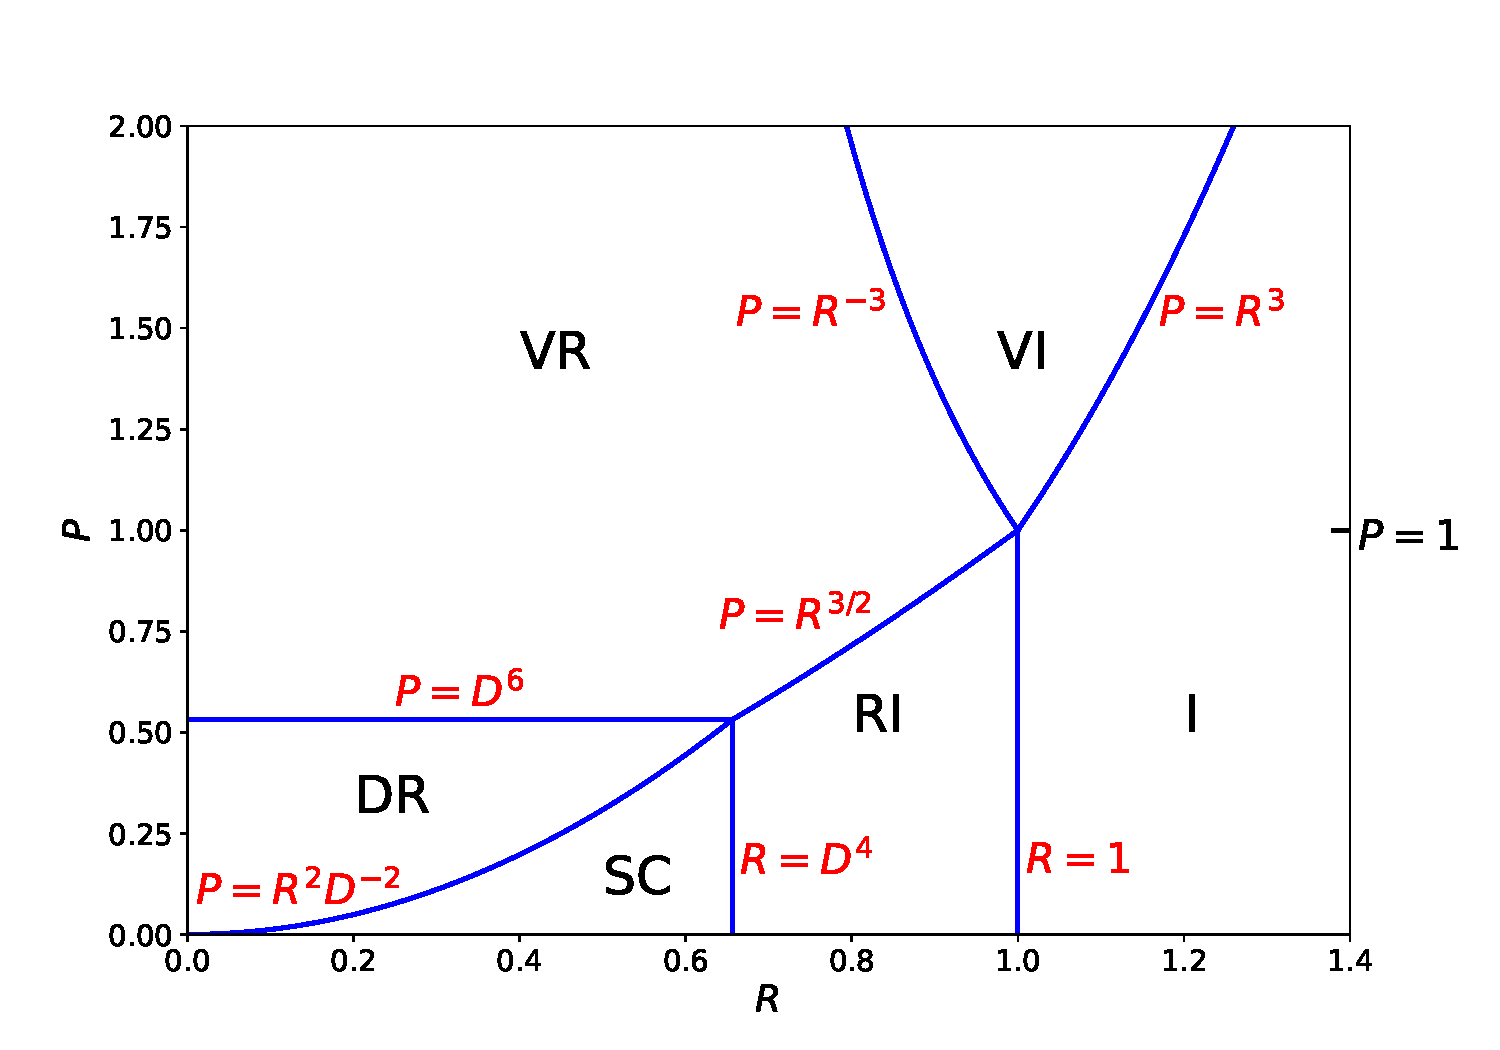
\includegraphics[width=1.\textwidth]{RegimeI.pdf}
\caption{Linear resonant plasma response regimes in $R$-$P$ space for the case $D = 0.9$. The various regimes are the diffusive-resisitive (DR), the semi-collisional (SC), the resistive-inertial (RI), the viscous-resistive (VR), the viscous-inertial (VI), and the inertial (I).}\label{f1}
\end{figure}

\begin{figure}
\centering
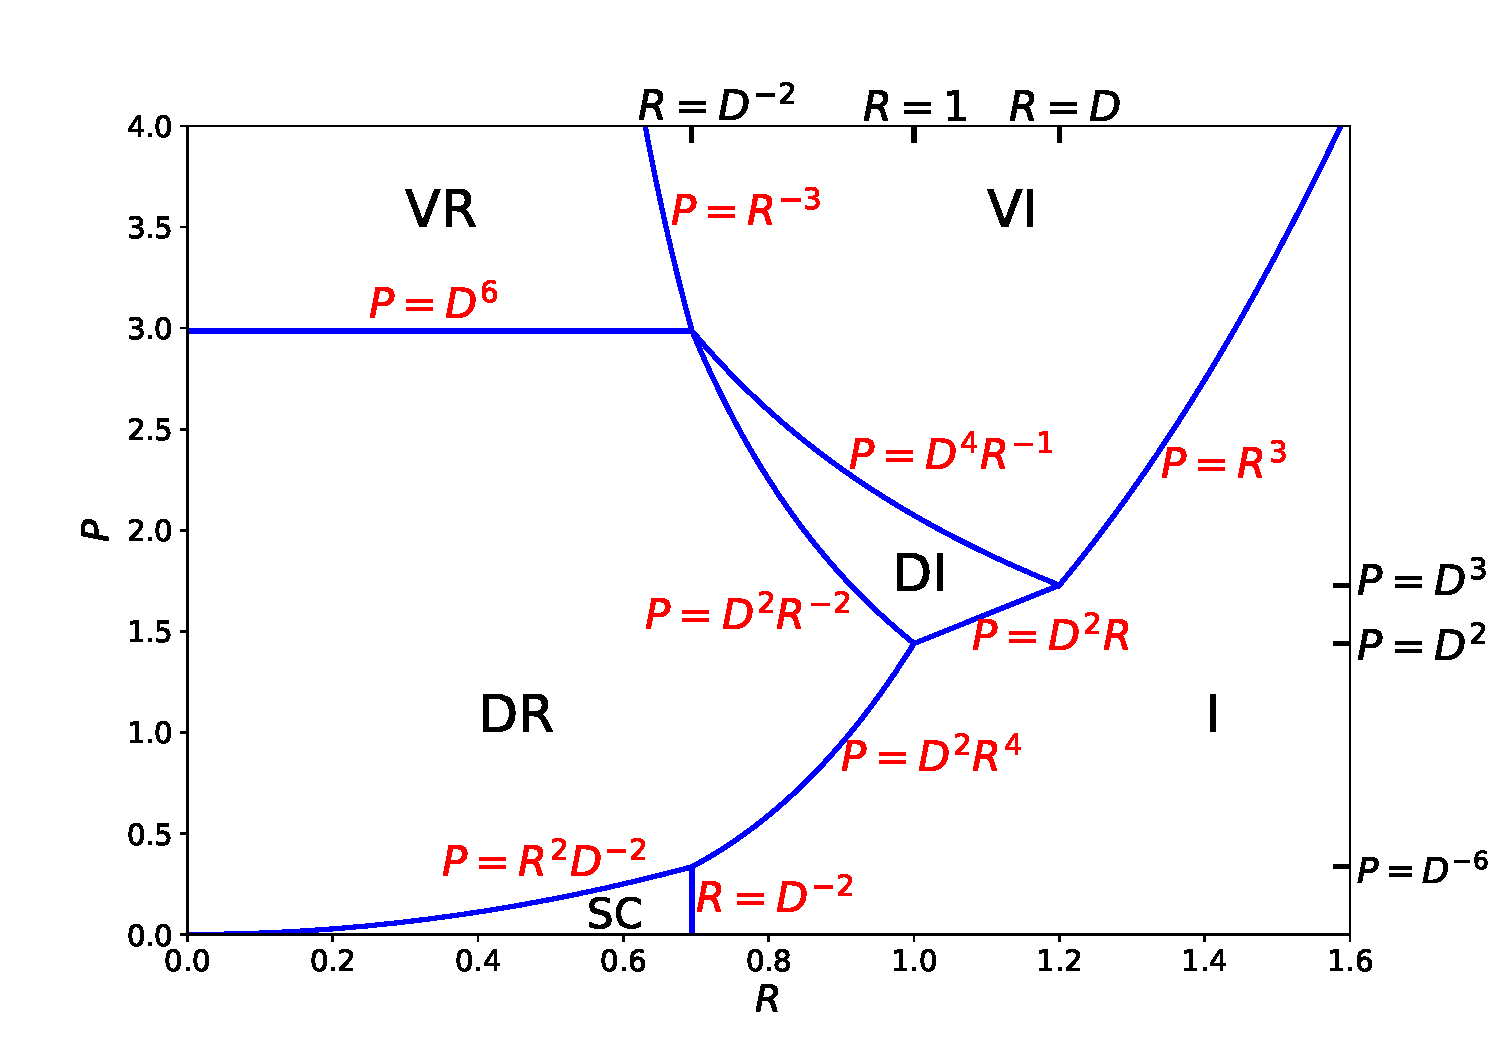
\includegraphics[width=1.\textwidth]{RegimeII.pdf}
\caption{Linear resonant plasma response regimes in $R$-$P$ space for the case $D = 1.2$. The various regimes are the diffusive-resisitive (DR), the semi-collisional (SC), the diffusive-inertial (DI), the viscous-resistive (VR), the viscous-inertial (VI), and the inertial (I).}\label{f2}
\end{figure}


\end{document}